%\documentclass[12pt,letter]{report}
\documentclass[12pt,oneside,openany,letter]{book}
\usepackage[colorlinks=true,bookmarksnumbered,linktocpage,pdftex]{hyperref}
\usepackage{hyperref}
\usepackage[activeacute,spanish]{babel}
\usepackage[utf8]{inputenc}
\usepackage{amsmath}
\usepackage{float}
\usepackage{epsfig}
\usepackage{graphicx}
\usepackage{titlesec}
\usepackage{multirow}
\usepackage{graphicx}
\usepackage{caption}
\usepackage{subcaption}
\usepackage{color}
\usepackage{calc}
\usepackage[nottoc]{tocbibind}
\usepackage{titletoc}
\usepackage{capt-of}
\usepackage{verbatim}
\usepackage[titletoc,title]{appendix}
\usepackage[left=3cm, right=3cm,top=3cm, bottom=2.5cm]{geometry}

\newcommand{\bigrule}{\titlerule[1mm]}
\definecolor{c1}{rgb}{0,0.5,0}
\definecolor{c2}{rgb}{0.9,.0,0}
\definecolor{c3}{rgb}{.465,.535,.605}%color del panel
\definecolor{c4}{rgb}{.6,.6,.6}%color de los botones del panel

\hypersetup{linkcolor=blue}                         
\hypersetup{citecolor=red}

%%%%FORMA DE LOS CAPITULOS SECCIONES...ETC%%%%%%

%========================================
% Formato de capítulos y secciones
%\newcommand{\esp}{\rule{0in}{3ex}} %para crear espacios en las tablas
\usepackage{titlesec}
\titleformat{\section}[hang]{\bfseries} {\Large\thesection}{12pt}{\Large}[{\titlerule[0pt]}]
 % Para hacer una línea debajo de cada sección
\titleformat{\chapter}[display] % cambiamos el formato de los capítulos
{\bfseries\Huge} % por defecto se usarán caracteres de tamaño \Huge en negrita
{ \filleft % texto alineado a la derecha
 \Large\chaptertitlename\ % "Capítulo" o "Apéndice" en tamaño \Large en lugar de \Huge
 \Large\thechapter} % número de capítulo en tamaño \Large
{0mm} % espacio mínimo entre etiqueta y cuerpo
{\filleft} % texto del cuerpo alineado a la derecha
[\vspace{0.5mm} \bigrule] % después del cuerpo, dejar espacio vertical y trazar línea horizontal gruesa



\setlength{\parskip}{10pt} %espacio entre párrafos
\makeatletter
\newcommand\figcaption{\def\@captype{figure}\caption}
\makeatother


%%%%%%%%%% NEW COMANDS %%%%%%%%%%%%%%%%%%%%%%%%%%%%%%%%%%%%%%%%%55

%%%%%%%%%%%%%%%%%%%%%%%%%%%%%%%%%%%%%%%%%%%%%%%%%%%%%%%%%%%%%%%%%%%%%%%%%%%%%%
\parindent0cm %Sangria
\parskip0.5cm %Espacio entre prrafos.
\baselineskip0.5cm
\begin{document}
\begin{titlepage}


\centering {\Large {\sc  ELVES: Fenómenos Luminosos Transitorios de la alta Atmósfera}}

\vfill

\centering {\Large \textbf{MSc Adriana Carolina Vásquez Ramírez} $^{\ast \circ }$}

\vfill

\centering {\Large \textbf{Director:} PhD Luis A. Núñez $^{\ast \circ }$}

\centering {\Large \textbf{Director:} PhD Roberto Mussa $^{\dagger }$}

\vfill

$\ast$  Grupo de Investigaci\'on en Relatividad y Gravitaci\'on - UIS \\
$\circ$ Grupo Halley de Astronom\'ia y Ciencias Aeroespaciales - UIS
\\
$\dagger$ INFN Sezione di Torino, Torino, Italia\\
\vfill

\centering {\Large Universidad Industrial de Santander\\Facultad de
Ciencias\\Escuela de F\'{i}sica\\2019}
\end{titlepage}

\tableofcontents
\listoffigures
%\listoftables
%\newpage


%%%%%%%%%%%%%%%%%%%%%%
%%%%% CHAPTER 1  %%%%%
%%%%%%%%%%%%%%%%%%%%%%
\chapter*{Introducción}\label{introduccion}
%empieza con la atmósfera, qué fenómenos ocurren ahí, por qué y con qué condiciones.
%todo lo que es física de relàmpagos (el papel de los rayos cósmicos en esto)
%hotspots de lightnings o tormentas alrededor del mundo (el fenómeno del catatumbo :3 )
%Breve explicación de qué son los TLEs (historia de la pagina 30-44 del libro )
%Enfásis en los ELVES



\chapter{Tormentas eléctricas}\label{tormentas}
Las tormentas eléctricas se producen en nubes densas de gran extensión vertical, conocidas como cumulonimbos, que se forman a partir del vapor de agua transportado por potentes corrientes de aire ascendente. Este fenómeno meteorológico se distingue por la presencia de rayos y truenos, que usualmente van acompañados de vientos y lluvias fuertes, o a veces de granizo o de nieve. 

Por encima de estas tormentas, a diferentes altitudes de la atmósfera, ocurren los denominados Eventos Luminosos Transitorios. Para explicar el origen de estos fenómenos es necesario conocer la dinámica de las tormentas, así como sus características y distribución global. En las secciones siguientes se describe la estructura de carga más simple de las tormentas eléctricas, los lugares donde se originan los rayos, así como su fenomenología, terminología y propagación en la atmósfera. También se muestra la distribución global y las redes de monitoreo de rayos alrededor del mundo.  

\section{Estructura de carga de las tormentas}
La estructura de carga ideal de las tormentas eléctricas está definida por el modelo tripolar estándar, donde la nube tiene un centro de carga negativa principal, uno de carga positiva principal y un centro de carga positiva inferior (ver figura \ref{fig:tormenta_modelo}). Frecuentemente aparece una cuarta región de carga negativa significativa llamada capa superior de apantallamiento, que expulsa las líneas de campo eléctrico producidas por las cargas de la tormenta eléctrica. Esta capa se forma debido a la mayor conductividad del aire limpio fuera de la nube, especialmente en la estratósfera sobre la tormenta \cite{DwyerUman2014}. 

Generalmente, el centro de carga negativa principal se encuentra en un rango de temperatura entre -10 y -25 $^{\circ}$C, independientemente de la altura del terreno debajo de la tormenta, donde la nube contiene tanto hielo como agua súper-enfriada. Por ejemplo, para las tormentas de verano en Florida y Nuevo México, estas temperaturas ocurren aproximadamente entre 6 y 8 km s.n.m \cite{DwyerUman2014}, mientras que en el caso de las tormentas invernales japonesas estas temperaturas se producen a altitudes mucho más bajas (alrededor de los 2 km s.n.m.), debido a que la atmósfera allí es más fría. 
Por otra parte, la región de carga positiva principal suele ser más difusa que la capa negativa principal y reside en la zona superior de la nube. Dependiendo de la altura de la tormenta, la carga positiva superior puede oscilar entre 8 y 15 km de altitud en las tormentas de verano, mientras que en invierno su grosor es de unos pocos km. La región positiva inferior se encuentra debajo de la capa principal negativa y el fondo de la nube visible; por ejemplo, en las tormentas de verano en Florida estaría por encima de los 2 km de altitud \cite{DwyerUman2014}. 

La estructura de carga en una tormenta eléctrica es en realidad más compleja que la que se muestra en la figura \ref{fig:tormenta_modelo}, puede variar de una tormenta a otra y en ocasiones es muy diferente de la estructura ilustrada, incluso a veces al revés, con la carga positiva principal en la parte inferior y la carga negativa principal en la parte superior. Además, las dos nubes aisladas de la figura \ref{fig:tormenta_modelo} podrían ser parte de varias tormentas contiguas e interactivas que comprenden sistemas de tormentas más grandes y complejos \cite{DwyerUman2014}. 

Las estructuras de carga dentro de las tormentas puede evolucionar a lo largo de su tiempo de vida debido a que los rayos pueden depositar y reorganizar la carga. En conjunto, la estructura de carga y, por lo tanto, los campos eléctricos de las tormentas eléctricas son complejos, dependiendo del tiempo, la ubicación y el tipo de tormenta. 

Como resultado, dado que las mediciones de campo eléctrico in situ sólo muestrean una pequeña parte de la tormenta, sin dar de ninguna manera una imagen completa del entorno del campo eléctrico, se debe tener cuidado al interpretar las observaciones utilizando un modelo específico de la estructura de carga \cite{DwyerUman2014}.

\begin{figure}
    \centering
    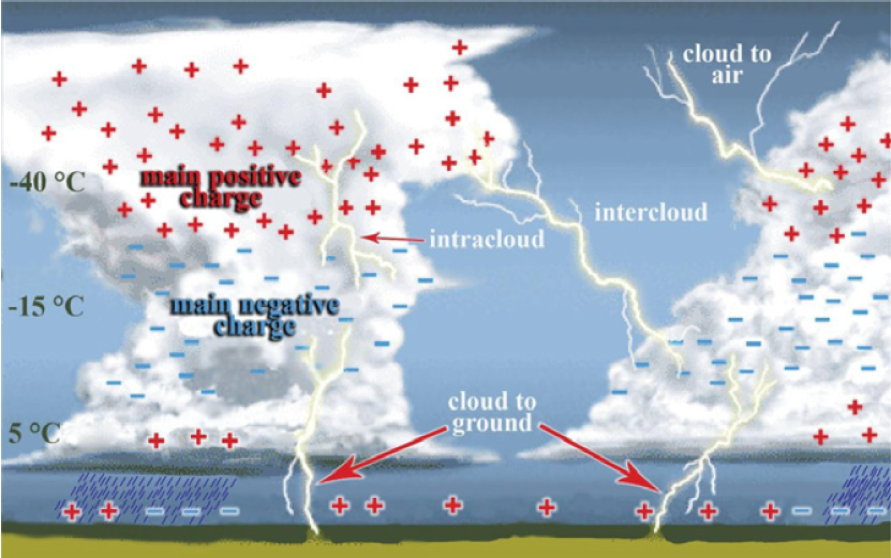
\includegraphics[scale=0.7]{figures/tormenta_modelo.png}
    \caption[Estructura de carga de dos tormentas simples aisladas según el modelo de tripolo.]{Estructura de carga de dos tormentas simples aisladas. Según el modelo de tripolo la parte superior de la nube está dominada por la carga positiva principal, seguida de la capa negativa principal y una pequeña capa de carga positiva en la parte más baja. Además se muestran algunos sitios donde se pueden producir los rayos: dentro de la nube (IC), de nube a tierra (CG), entre dos nubes (CC) e incluso de nube al aire (CA). Tomado de \cite{DwyerUman2014}.}
    \label{fig:tormenta_modelo}
\end{figure}

\subsection*{Mecanismos de carga de las nubes}

Usualmente, los mecanismos de carga de las nubes se clasifican en procesos inductivos y no inductivos. En el proceso inductivo, el campo eléctrico vertical existente induce la polarización de cargas en hidrometeoros suspendidos. Los hidrometeoros, son cualquier producto de condensación o deposición de vapor de agua atmosférica, ya sea que se forme en la atmósfera libre o en la superficie de la tierra, también, cualquier partícula de agua soplada por el viento desde la superficie de la tierra. Wilson (1929) hipotetizó que las gotas de lluvia en presencia de un campo positivo capturan iones negativos. 

El campo eléctrico se mejora aún más debido al refuerzo del campo del
separación gravitacional de las gotas con carga negativa que caen y de la carga neta positiva en iones localizados hacia arriba en la nube. El proceso de carga dependerá del ritmo de producción de iones en la atmósfera inferior y la posibilidad de desintegración de una gota debido a una carga aislada (Taylor 1964). Latham y Mason (1962) proveyeron servicios de matemáticas descripción de la carga de granizo en un campo eléctrico polarizado. Abbas y Latham (1967) demostró que una gota que lleva una carga negativa inicialmente pequeña adquiere una una carga negativa cada vez mayor con un campo eléctrico en aumento y alcanza un valor crítico. que depende del radio de la gota, independientemente del potencial y del campo eléctrico. Taylor (1964) mostró que este valor crítico es aproximadamente 0,38 veces mayor que el requerido para desintegrarse. una gota cargada. Además, el campo eléctrico máximo que podría ser generado por este en una nube con la ionización predominante en la troposfera no puede exceder de ~ 600 V m-1 (Chalmers 1962). Los rayos cósmicos generaron iones en la atmósfera inferior también juegan un papel clave en las etapas iniciales del mecanismo de convección para la electrificación de nubes (Vonnegut 1963). Sartor (1967) propuso 


\section*{Mediciones de campo eléctrico dentro de la tormenta}



\section{Lugares de iniciación de los rayos}
El problema de iniciación de los rayos dentro de las nubes, es uno de los mayores misterios de las ciencias atmosféricas y la física de los rayos. El problema radica en el hecho de que en décadas de mediciones de campo eléctrico, realizadas directamente en el interior de las nubes, no se han logrado encontrar fuerzas de campo eléctrico lo suficientemente grandes como para producir una chispa, incluso cuando se tienen en cuenta los efectos de la reducción de la densidad del aire y la presencia de partículas de agua y hielo. Sin embargo, rutinariamente se observan chispas muy grandes que se producen dentro de las tormentas eléctricas en forma de rayos. Esto sugiere que hay algo mal en las mediciones o en la comprensión de cómo ocurren las descargas eléctricas en el entorno de una tormenta \cite{DwyerUman2014}. Para que la ruptura dieléctrica ocurra dentro de las tormentas eléctricas se requiere un campo eléctrico de unos 23 kV/cm \cite{GurevichEtal2009}, pero el campo eléctrico medido y simulado es un orden de magnitud menor a este valor \cite{MarshallEtal2005, DwyerEtal2006, StolzenburgEtal2007}. Se cree que los rayos cósmicos (RCs) pueden estar involucrados en la formación y las tasas de cubrimiento de nubes en la Tierra, aunque el mecanismo físico que establece este vínculo sigue siendo poco entendido. 

La ionización en la troposfera y en la estratosfera se produce principalmente por los rayos cósmicos mientras que en la ionosfera la radiación solar ultra-violeta

Solar Extreme Ultraviolet (EUV) is solar radiation that covers the wavelengths 10 – 120 nm of the electromagnetic spectrum. It is highly energetic and it is absorbed in the upper atmosphere, which not only heats the upper atmosphere but also ionizes it, creating the ionosphere. Solar EUV radiation changes by a factor of ten over the course of a typical solar cycle. This variability produces similar variations in the ionosphere and upper atmosphere. Solar EUV variations are one of the three primary drivers of ionospheric variability.

Los RCs son partículas de alta energía procedentes del espacio exterior, que al interactuar con la atmósfera cambian la concentración de iones atmosféricos y la troposfera, a través de la modulación del flujo de corriente en el circuito global eléctrico. Los rayos cósmicos que entran en la atmósfera producen ionización y por lo tanto afectan la conductividad eléctrica atmosférica de la Tierra, el circuito eléctrico global, las tasas de nucleación en las nubes, las descargas de rayos, entre otras \cite{KumarEtal2018}. Los resultados iniciales del experimento CLOUD (Cosmics Leaving OUtdoor Droplets) del CERN son alentadores en cuanto al estudio de la posible influencia de las rayos cósmicos en las nubes (duplissy 2010). Las medidas respaldan la formación adicional de CCN pero su contribución no está cuantificada. 

Svensmark 1997 y Marsh 2000 reportaron una correlación entre los rayos cósmicos y nubes de baja altitud (<3 km) alrededor del mínimo de RCs de 1990. Por otra parte, Kumar et al (2017) demostró que la cobertura nubosa de bajo nivel (presión > 680 h Pa) está positivamente correlacionada con el flujo de rayos cósmicos galácticos, utilizando mediciones en la Antártida en condiciones de buen tiempo. La correlación máxima es del 36\% durante el mínimo solar largo entre 2007-2009 \cite{KumarEtal2018}. 

Existen varios mecanismos propuestos que involucran rayos cósmicos: 
Gurevich y Zybin(2001, 2005) propusieron que el runaway breakdown mechanism operando a un voltaje más bajo (2.16 kV/cm) donde se involucra el paso de partículas de alta energía, los rayos cósmicos, a través de la tormenta  \cite{KumarEtal2018}. 

otro mecanismo de crs pagina 866 de \cite{KumarEtal2018}

Tomando en cuenta la estructura ideal de carga de las nubes discutida anteriormente en la figura \ref{fig:tormenta_modelo}, se puede notar  que no existe una sola ubicación para la iniciación de los rayos, puesto que no hay una estructura única de carga para las tormentas eléctricas. Aún así se han observado ciertos patrones que ayudan a clasificar las descargas eléctricas en una tormenta en dos categorías: 
\begin{itemize}
    \item Las que unen la brecha entre la carga de la nube y la tierra;
    \item y las que no. 
\end{itemize}

Las primeras se conocen como descargas de nube a tierra, denotadas por CG, y se clasifican en cuatro tipos dependiendo del signo de la carga eléctrica y la dirección de propagación que lleva el ``líder inicial" (ver detalles en la sección \ref{fenomenologia}). Las segundas se dividen dependiendo del lugar donde se producen: dentro de la nube (denotado en inglés como IC), entre dos nubes (CC) y de la nube al aire (CA). Este grupo representa la mayoría de todas las descargas de rayos, siendo las IC las más comunes de todas las formas, seguidas de las CC y de las CA. Por otra parte, un sistema típico de tormenta eléctrica pequeña produce un relámpago CG cada 20-30 s durante 40-60 min y cubre un superficie típica de 100-300 km2. Los sistemas de tormentas grandes pueden producir más de un flash a tierra cada segundo, en áreas cien veces más grandes \cite{DwyerUman2014}. 

\section{Fenomenología de los rayos}\label{fenomenologia}
Los rayos se pueden definir como una chispa eléctrica muy larga, que generalmente rondan entre 5 y 10 km de longitud, con algunos casos extremos de 100 km. Estos fenómenos son los más impresionantes y comunes en geofísica, pues producen la luz más brillante (relámpago) y el sonido más fuerte (trueno) en la Tierra. La duración temporal va desde ... . El rayo más largo registrado hasta ahora fue de .... y tantos segundos... A nivel mundial se generan alrededor de 9 millones de descargas al año, lo que se traduce a una tasa promedio de $6$ rayos por $\text{Km}^{2}$ por año \cite{DwyerUman2014}. 

El proceso de transferencia de la carga primaria ocurre a través de las colisiones entre partículas de granizo blando y de pequeños cristales de hielo. El granizo es lo suficientemente pesado como para caer o permanecer inmóvil en las corrientes ascendentes de la tormenta; mientras que los cristales de hielo son lo suficientemente ligeros para dejarse llevar hacia arriba por esas corrientes. Para generar las cargas principales del modelo de tripolo de las tormentas, las interacciones de granizo-hielo deben producirse en altitudes donde la temperatura está alrededor de $-10\,^{\circ}$C a $-20\,^{\circ}$C \cite{DwyerUman2014}. 

aqui
\begin{figure}
    \centering
    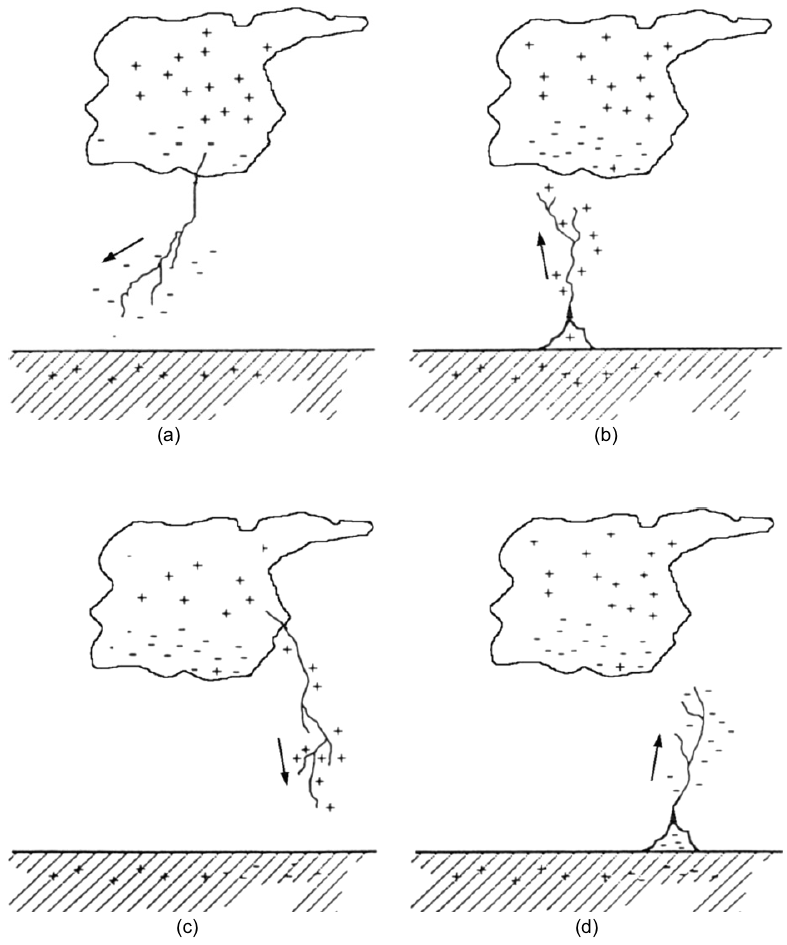
\includegraphics[scale=0.5]{figures/CG4.png}
    \caption{Caption}
    \label{fig:CG4}
\end{figure}

En la figura \ref{fig:CG4} se muestran los 4 tipos de CG.  


De los CG, los más comunes son los que van hacia abajo llevando carga negativa, se describen a continuación (figura 1.3 del \cite{DwyerUman2014})

\section{Distribución global y monitoreo de los rayos}

%WWLLN
%NASA
%Auger
%Proyecto relámpago

La tormentas en la Tierra se producen mayormente dentro de las regiones tropicales, es decir, entre $\pm 30^{\circ}$ de latitud respecto al ecuador, debido al máximo calentamiento solar que ocurre en los trópicos y a las células de circulación atmosférica general de Hadley. Estas son células de circulación cerrada de la atmósfera terrestre, donde el calor es transportado en un movimiento celular con el aire ascendiendo por convección en las regiones ecuatoriales y desplazándose hacia las latitudes superiores por las capas altas de la atmósfera. El ascenso del aire caliente en el ecuador está acompañado de la formación frecuente de tormentas convectivas en la llamada zona de convergencia intertropical. Además, la actividad global se concentra más sobre las regiones continentales (las Américas, Africa y el sureste de Asia) que sobre los océanos, debido a que el calentamiento diario sobre la superficie de la tierra es mayor que en la superficie de los océanos. 

El efecto integrado de las tormentas eléctricas globales y otras nubes electrificadas se puede estudiar a través del circuito eléctrico global atmosférico (CEGA), que se define como el curso continuo de la electricidad atmosférica entre la ionósfera (a 80 km de altitud) y la superficie terrestre. Se estima que las tormentas globales cargan negativamente la superficie de la Tierra con un valor medio de 500 kC y el potencial eléctrico medio generado entre estas capas es de 250 kV \cite{FullekrugEtal2006}. En climatología la representación más precisa hasta la fecha del total de relámpagos en todo el planeta es la base de datos de la HRAC (High Resolution Annual Climatology), que contiene las observaciones realizadas por dos satélites de la NASA: el OTD y el LIS. El OTD (Optical Transient Detector) fue el primer instrumento diseñado específicamente para detectar rayos desde el espacio durante el día y la noche entre los años 1995 y 2000. Este fue un prototipo del LIS, Lightning Imaging Sensor, que fue lanzado en 1997 y recompiló información hasta abril del 2015. A partir de estos 20 años de datos se reconfirmó que la tasa media global de rayos es de 46/s, variando desde 35/s en austral summer hasta 60/s en boreal summer. Además se establecieron los sitios de producción de rayos más activos del planeta y los 10 primeros se muestran en la tabla 

\begin{table}[]
\begin{tabular}{|c|c|c|c|c|}
\hline
\textbf{Puesto mundial} & \textbf{FRD} & \textbf{Latitud} & \textbf{Longitud} & \textbf{Sitio}               \\ \hline
1                       & 232.52       & 9.75             & -71.65            & Lago de Maracaibo, Venezuela \\ \hline
2                       & 205.31       & -1.85            & 27.75             & Kabare, R.D. del Congo       \\ \hline
3                       & 176.71       & -3.05            & 27.65             & Kampene, R.D. del Congo      \\ \hline
4                       & 172.29       & 7.55             & -75.35            & Cáceres, Colombia            \\ \hline
5                       & 143.21       & -0.95            & 27.95             & Sake, R.D. del Congo         \\ \hline
6                       & 143.11       & 34.45            & 72.35             & Daggar, Pakistan             \\ \hline
7                       & 138.61       & 8.85             & -73.05            & El Tarra, Colombia           \\ \hline
8                       & 129.58       & 5.25             & 9.35              & Nguti, Cameroon              \\ \hline
9                       & 129.50       & 0.25             & 28.45             & Butembo, R.D. del Congo      \\ \hline
10                      & 127.52       & -1.55            & 20.95             & Boende, R.D. del Congo       \\ \hline
\end{tabular}
\end{table}



en la figura se muestran los top 10 FRD (flash rate density) \cite{AlbrechtEtal2016}. 
\begin{figure}
    \centering
    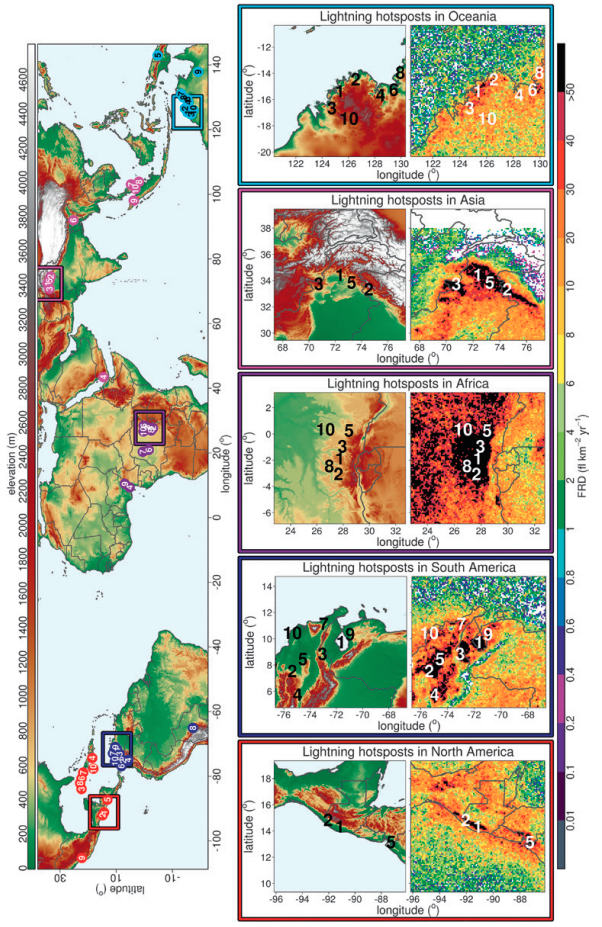
\includegraphics[scale=0.7]{figures/hotspots.png}
    \caption{Caption}
    \label{fig:my_label}
\end{figure}





%The lightning detection is based basically on two types of systems. On the one hand optical observation from space, as the Optical Transient Detector (OTD) [97] or the Lightning Imaging Sensor (LIS) [98] and on the other hand the detection of the radio noise generated by the lightning in the VLF/LF band with multiple antennas and a time of arrival reconstruction, as National Lightning Detection Network (NLDP) [99], the European lightning location system (EUCLID) [100] or the World Wide Lightning Location Network (WWLLN) [101] which is described in section 8.3 in more detail.


%%%%%%%%%%%%%%%%%%%%%%
%%%%% CHAPTER 2  %%%%%
%%%%%%%%%%%%%%%%%%%%%%
\chapter{Eventos Luminosos Transitorios en la alta atmósfera}\label{TLEs}
Los Eventos Luminosos Transitorios, denominados como TLE, son emisiones cortas de luz que ocurren encima de las tormentas eléctricas, en las capas más altas de la atmósfera, es decir, en la estratósfera, la mesósfera y en la parte baja de la ionósfera. Estos eventos se originan a partir de las descargas eléctricas que ocurren entre las nubes, o entre las nubes y el suelo \cite{DwyerUman2014}. Hasta ahora, se han reportado los siguientes tipos de TLEs: Sprites, Blue Starters, Blue Jets y Gigantic Jets, Elves y Halos. La dinámica de estos fenómenos electromagnéticos, que involucra corrientes eléctricas, ondas electromagnéticas y gases ionizados, aún no se entiende por completo \cite{Maiorana2014}.

Los TLEs se empezaron a reportar hace más de 130 años, cuando MacKenzie y Toynbee describieron en 1886 lo que hoy sería conocido como un \textit{Giagantic Jet}. A Corliss (1977), Vaughan Jr. y Vonnegut (1989), y Vonnegut
(1980), se les atribuye la compilación de numerosos testimonios creíbles de testigos oculares. Las primeras imágenes de un sprite fueron capturadas cuando el profesor J.R. Winckler y sus estudiantes estaban probando un \textit{low-light television} (LLTV) para un próximo vuelo con cohetes de investigación en 1990. El video reveló un ``rayo de calor" distante, y columnas gemelas brillantes de luz que se extendían decenas de kilómetros en la atmósfera. Este tipo de ``rayo ascendente" llamó la atención del programa de vuelos espaciales tripulados de los Estados Unidos, debido a los varios encuentros desafortunados de sus naves espaciales con rayos. A partir de esto se instauró un programa de mapeo de rayos a meso-escala, introduciendo cámaras similares a los LLTV en el Transbordador Espacial. En este caso los vídeos revelaron un brillo transitorio que se iba ensanchando --seguramente un elves-- y más de una docena de ``rayos ascendentes" sobre la tormenta. A partir de 1993 la NASA comenzó a financiar investigaciones terrestres y aéreas en este campo. En ese período se instaló el mismo LLTV de Winclker en la Estación de Campo Yucca Ridge de la FMA, donde se detectaron alrededor de 250 eventos durante varias horas por encima de una tormenta ubicada a 400 Km al este. En 1994, grupos de la Universidad de Alaska y de la FMA notaron que estos eventos tenían asociadas señales características de audio de muy baja frecuencia (VLF). Ese mismo año montaron la campaña aérea que produjo las primeras imágenes a color de los sprites y aparecieron inesperadamente los \textit{blue jets}. A partir de la campaña YRFS que se llevó a cabo entre 1994 y 1995, se hizo evidente la correlación entre los sprites y los rayos tipo +CG. De los 10.000 eventos confirmados sólo algunos sprites fueron relacionados con rayos -CG \cite{FullekrugEtal2006}. 

\begin{figure}
    \centering
    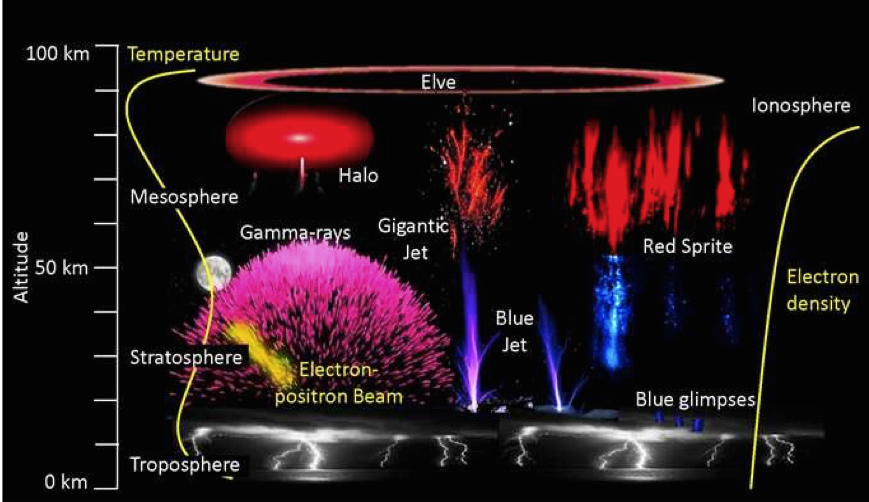
\includegraphics[scale=0.75]{figures/tle_and_tgf.png}
    \caption[Fenómenos de la atmósfera superior generados por tormentas eléctricas]{Fenómenos de la atmósfera superior generados por tormentas eléctricas, incluyendo destellos de rayos gamma terrestres (TGFs) y emisiones luminosas transitorias (TLEs). Las descargas eléctricas que incluyen ``destellos azules'' en la parte superior de las tormentas eléctricas, blue jet, gigantic jet, red sprite, halos, y elves (Tomado de \cite{Gaskill2018}).}
    \label{fig:tle_and_tgf}
\end{figure}

Por otra parte, los elves fueron confirmados ópticamente por primera vez en 1995, por Fukunishi et al (1996) en la campaña YRFS. En 1993 Taraneko et al habían predicho este fenómeno, describiéndolo como un brillo intenso muy breve ($<1$ms) producido en la base de la ionosfera asociado con el Pulso Electromagnético (EMP) de un rayo. Los programas ópticos de la YRFS y el Laboratorio Langmuir de Nuevo Mexico, revelaron que lo que muchos de los primeros observadores pensaban que era un elves, en realidad se trataba del halo que precede a algunos, pero no a todos los sprites \cite{FullekrugEtal2006}. 

Para un estudio más fino de la estructura espacial y temporal de los sprites, elves y halos se utilizaron --y aún se emplean-- una variedad de sensores fotométricos, como el ``ojo de mosca", cámaras de alta velocidad, cámaras de alta resolución e imágenes telescópicas de alta velocidad\cite{FullekrugEtal2006}. A partir de estas observaciones se estimaron las características de los TLEs, como la altitud a la que se producen, su tiempo de vida, tamaño, forma, brillo y la tasa de producción en una tormenta típica. En la figura \ref{fig:tle_and_tgf} se muestran los diferentes fenómenos de la atmósfera superior producidos por tormentas eléctricas, incluyendo los destellos de rayos gammas terrestres (TGF) y los TLEs. En ésta se puede observar la altitud característica de cada evento, así como el tamaño referencial de unos respecto a otros. 

En las secciones siguientes se describen las características más conocidas hasta ahora sobre estos fenómenos, como su estructura, el tiempo de duración, altitud y frecuencia con la que ocurren, brillo y otras. 

\section{Sprites} 
Los sprites son grandes ráfagas de luz tenue producidas encima de las tormentas eléctricas, que consisten en una cascada de plasma electrificado de color rojizo en su región superior, con ramificaciones azuladas en su parte inferior. El origen de sus filamentos eléctricos generalmente se produce alrededor de los 70 a 75 Km de altitud \cite{FullekrugEtal2006}. Estas ramas altamente estructuradas, suelen propagarse primero hacia abajo, seguidas de una expansión hacia arriba en luminosidad, con un resplandor más difuso en la parte superior. Generalmente, los filamentos no se extienden más allá de los 40 Km \cite{FullekrugEtal2006}. 

Todos los sprites son visualmente diferentes, pero se pueden clasificar según su forma en: los tipo columna (c-Sprites) y los tipo zanahoria (z-Sprites). Los c-Sprites suelen ser muy estrechos, con un ancho del orden de 1 km. Son casi continuos, es decir, casi verticales, con filamentos que se extienden hacia abajo y hacia arriba. Estos pueden aparecer en grupos de una docena o más sprites, repartidos en varias decenas de kilómetros. El clásico sprite de ``zanahoria" tiene grupos de filamentos que se estrechan hacia abajo con elementos que se ensanchan hacia afuera en la parte superior \cite{FullekrugEtal2006}. Todavía se desconocen los mecanismos que producen estas formas, así como los detalles de su evolución. En la figura \ref{fig:sprite_evolution} se muestra la evolución temporal de un z-sprite típico.

\begin{figure}[h!]
    \centering
    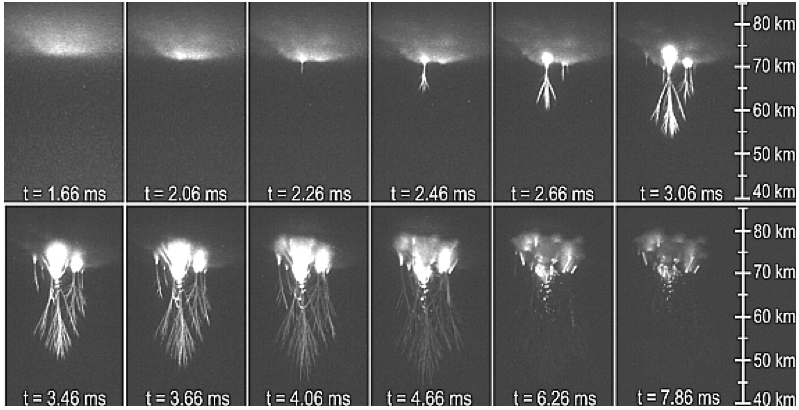
\includegraphics[scale=0.8]{figures/sprite_evolution2.png}
    \caption[Evolución temporal de un sprite]{Imágenes del desarrollo de la estructura de un z-sprite típico. Las etiquetas de tiempo se refieren al inicio del return stroke del rayo \cite{CummerEtal2006}.}
    \label{fig:sprite_evolution}
\end{figure}

Los sprites ocurren sólo después de las descargas de relámpagos CG con un líder positivo. Estos fenómenos pueden durar desde algunos milisegundos hasta decenas de milisegundos, tiempo suficiente para ser capturados por cámaras, o incluso por el ojo humano \cite{Maiorana2014}. Se estima que el brillo inherente de los sprites está alrededor de 1.0 MR, con algunos casos raros donde pueden alcanzar desde 10 MR hasta 30 MR \cite{FullekrugEtal2006}. 

Las diferentes medidas realizadas en la superficie sugieren que, en una tormenta típica, se tiene 1 sprite cada minuto. Un caso interesante son las Altas Llanuras de los Estados Unidos, donde después de la aparición inicial, los sprites usualmente continúan saliendo por varias horas. En ocasiones, estas tormentas han producido de 400 a 750 sprites en 4-5 horas \cite{FullekrugEtal2006}.

\section{Blue starters, blue jets y jets gigantes}
Los blue starters y jets son rayos que salen del tope de las nubes hacia arriba, se extienden hasta unos 30 a 40 Km de altitud y luego se desvanecen. Estos eventos tienen forma de cinta, son de color azul y suelen ser más brillantes que los sprites ($>1$ MR). Suelen propagarse con velocidades alrededor de $10^5$ m/s y su tiempo de vida ronda en los 300 ms \cite{DwyerUman2014}. Por otro lado, se tienen los jets gigantes que pueden llegar hasta los 70 Km de altitud. La forma de un jet gigante es más compleja que uno simple, a veces se describen como la mezcla de un jet y un sprite, debido a que su parte baja es cónica como un jet y luego se dispersa en un brillo difuso y tenue, de un tono rojizo como un sprite. 

Los blue jets ocurren más o menos con la misma frecuencia que los sprites, mientras que los jets gigantes son bastante raros, con una tasa de 13 en tres años. Estos no están asociados con descargas de rayos dirigidos hacia abajo sino que pueden contener un flujo de partículas aceleradas que podría estar relacionada con los TGFs \cite{Maiorana2014}. Recientemente, investigadores de Estados Unidos y de la Universidad de Cataluña \cite{VanEtal2019}, capturaron con cámaras de alta velocidad el nacimiento y las etapas de evolución de jets gigantes en la costa norte colombiana. En la figura \ref{fig:gigantic_jets_colombia} se aprecia claramente la evolución temporal de un jet gigante con sus cuatro etapas: el jet líder, el jet completamente desarrollado, el jet de seguimiento y el líder final. 

\begin{figure}
    \centering
    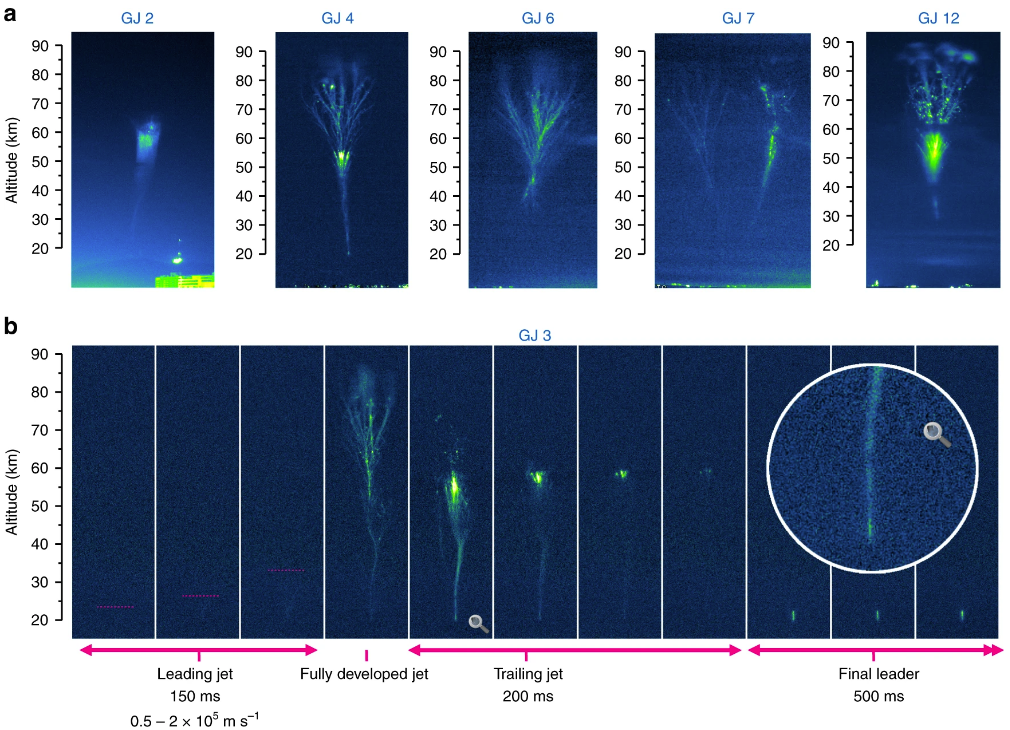
\includegraphics[scale=0.45]{figures/gigantic_jets_colombia.png}
    \caption[Jets gigantescos capturados en la costa norte de Colombia]{a) Cinco jets gigantescos capturados en la costa norte de Colombia: Santa Marta (GJ 2-4), Barranquilla (GJ 7) y Cartagena (GJ 12). b) Etapas de la evolución de un jet gigante grabadas con una cámara de 2.3 megapíxeles a 20 imágenes por segundo, se puede observar el jet líder en los primeros 150 ms seguido del jet completamente desarrollado, el jet de seguimiento y el líder final \cite{VanEtal2019}.}
    \label{fig:gigantic_jets_colombia}
\end{figure}

\section{Elves}
Un elves es un disco toroidal de luz roja de rápida expansión, que se genera en la parte baja de la ionosfera (la altitud está entre los 80-100 Km). Típicamente son generados por el pulso electromagnético (EMP) de una descarga -CG y su diámetro puede extenderse hasta más de 300 Km. El EMP se propaga como una onda esférica desde la base del canal del rayo, intersectando la ionosfera inferior como un anillo que se expande más rápido que la velocidad de la luz en ese medio. El campo eléctrico del EMP produce la calefacción de electrones libres, aumentando las excitaciones inducidas por colisión, la ionización y las emisiones de luz óptica \cite{FullekrugEtal2006}.

Los elves están asociados a las descargas -CG que tienen corrientes de pico más altas que los rayos que producen los sprites, es decir, mayor a 80 kA. A partir de los datos tomados desde la tierra, se tiene que los sprites y los elves ocurren entremezclados en las mismas tormentas, aunque la proporción varía considerablemente de una tormenta a otra. Es raro tener sólo elves o sólo sprites en una tormenta dada \cite{FullekrugEtal2006}. Por otra parte, las observaciones de la misi\'on espacial ISUAL, sugiere que los elves son uno de los TLEs más comunes, superando en número a los sprites de 9 a 1. Además, los elves ocurren con más frecuencia sobre los océanos, posiblemente debido a que los rayos con corrientes de pico altas son más comunes sobre los océanos que sobre la tierra \cite{DwyerUman2014}. 

El nombre ELVES era originalmente un acrónimo de Emission of Light and Very low frequency perturbations due to Electromagnetic pulse Sources, aunque ahora pocos autores mencionan este nombre completo \cite{DwyerUman2014}. Estos fenómenos pueden ser tan brillantes como un sprite típico (∼1MR) pero su duración, de algunas decenas de microsegundos, hace que sean imperceptibles para el ojo humano y difíciles de detectar usando sistemas de vídeo. Es por esto que generalmente se detectan a partir de arreglos de fotómetros, con resoluciones temporales alrededor de los 0.3 ms \cite{Maiorana2014}. En la figura \ref{fig:elves_photo} se muestra una foto impresionante de un elve acompañado por tres sprites, tomada por el astrónomo Timo Kantola que corrió con la suerte de capturar esta escena. En la sección \ref{deteccion} se resume cómo  los grupos más resaltantes logran la detección de elves con sus respectivos instrumentos. 
\begin{figure}
    \centering
    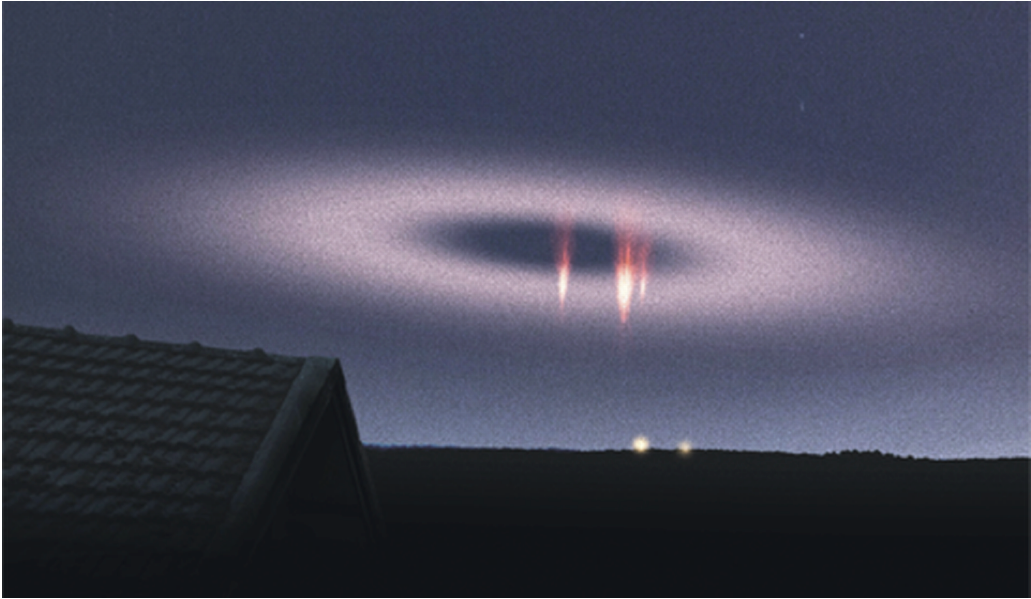
\includegraphics[scale=0.65]{figures/elves_photo.png}
    \caption[Foto de un elve tomada por el astrónomo Timo Kantola]{Foto de un elve junto a tres sprites tomada por el astrónomo Timo Kantola, en Pieksämäki Finlandia.}
    \label{fig:elves_photo}
\end{figure} 

%detalles de la inonosfera ya que ahí se forman los elves
%pulsos electromagnéticos y su propagación en la atmósfera
%mecanismos de producción de elves con los lightnings 

\section{Halos}
Son emisiones de luz difusa en forma de disco, que ocurren dentro de un campo eléctrico casi-estático como los sprites. Al principio estos discos se confundían con elves y como aparecían junto a los sprites solían llamarlos \textit{sprelves}. Ahora se sabe que los halos pueden aparecer junto con los sprites o por sí solos. Además su diámetro es mucho menor que el de los elves --máximo de 100 Km-- y su duración es mayor (alrededor de 1 milisegundo). Estos eventos se producen por debajo de los elves, entre los 65 y 80 Km de altitud. Los videos de alta velocidad (Armstrong y Lyons, 2000; Stanley et al., 1999; Stenbaek-Nielsen et al., 2000) han demostrado que el halo es un resplandor amorfo descendente en forma de lente que se inicia típicamente uno o dos milisegundos después del golpe de retorno (return strokes), y persiste de uno a tres milisegundos. Su brillo ronda entre los 0.5 y 1 MR \cite{FullekrugEtal2006}.

%\section{Elves en el Observatorio Pierre Auger}

%%%%%%%%%%%%%%%%%%%%%%
%%%%% CHAPTER 3  %%%%%
%%%%%%%%%%%%%%%%%%%%%%
\chapter{Detección global de los Elves}\label{deteccion}
La primera observación clara de un elves se hizo a partir de una cámara de alta velocidad a bordo del Transbordador Espacial en su misión STS-41 (1990). Esta cámara es sensible a longitudes de onda entre los 360 y 720 nm, con un máximo en 440 nm. Una simple molécula de nitrógeno ionizada emite luz a 427nm y 391nm, es decir, cerca al pico de sensibilidad de la cámara. Estos dispositivos son lo suficientemente sensibles para detectar las emisiones de luz en el aire; el vídeo fue grabado en formato blanco y negro, con una resolución temporal de una sesentava parte de un segundo ($\approx 17$ ms). 


La imagen fue mejorada, restando el fondo y expandiendo el extremo superior de la escala de grises, para determinar si el aumento en el brillo de la imagen era una fluctuación aleatoria o la luminosidad de una descarga de rayo. Este evento luminoso transitorio fue observado a una altitud alrededor de los 95 km, en coincidencia con un rayo producido en una tormenta oceánica tropical directamente debajo del elves \cite{BoeckEtal1992}.  

Luego estos fenómenos fueron estudiados a partir de arreglos lineares de fotómetros verticales y horizontales con un tiempo de resolución mejorado a $40\,\mu$s. [revisar estas 3–5]. 

Satellite data on ELVES have been acquired by the ISUAL/Formosat-2 mission, from 2004 to
2007, using conventional and multianode PMTs, with time resolutions of 100 and 50 μs, respectively [6]. These data allowed to conclude that ELVES develop on oceans or coastal regions ten times more frequently than on land. 
While future space missions (Taranis [7], Firefly [8], JEM-EUSO [9]) have included the observation of ELVES in their physics program, we want to show that the Pierre Auger Observatory can be transformed in the best ground based instrument for the observation of such events in the near UV band, with a simple set of modifications of the current triggering
scheme.

%más detalles sobre los elves 
%tipos de elves: simple, doble, multiple 
%detectores alrededor del mundo 
%enfasis en el FD de Pierre Auger

\section{Elves en el Observatorio Pierre Auger}

El Observatorio Pierre Auger es un 
\bibliographystyle{unsrt}
\bibliography{monografia}

\end{document}